% !Mode:: "TeX:DE:UTF-8:Main"
% arara: pdflatex
% arara: pdflatex
% xarara: convert: {density: 160, otheroptions: -dispose previous -delay 10 -loop 0, format: gif}
%magick -density 160 -delay 60 -loop 0 goodbye.pdf goodbye.gif
\PassOptionsToPackage{x11names}{xcolor}

\documentclass{beamer}
\usepackage{tikzlings,tikzducks,xfp}
\usetikzlibrary{overlay-beamer-styles}
\setbeamertemplate{navigation symbols}{}

\newsavebox\bondducks
\tikzset{
  linea/.style={white, line width=4pt,},
  pics/microph/.style={code={
        \draw[black, line width=.2em, rounded corners=1.7ex]
            (-.85em,4.5ex) -- (-.85em,2ex) -- (.85em,2ex) -- (.85em,4.5ex);
        \fill[black]
            (-.6em,5ex) to[rounded corners=1.2ex]
            (-.6em,2.5ex) to[rounded corners=1.2ex] (.6em,2.5ex)
            -- (.6em,5ex) to[rounded corners=.2ex] ++(-.85em,0) to[rounded corners=.2ex] ++(0,.35ex) -- ++(.85em,0)
            -- (.6em,5.5ex) to[rounded corners=.2ex] ++(-.85em,0) to[rounded corners=.2ex] ++(0,.35ex) -- ++(.85em,0)
            -- (.6em,6ex) to[rounded corners=.2ex] ++(-.85em,0) to[rounded corners=.2ex] ++(0,.35ex) -- ++(.85em,0)
            -- (.6em,6.5ex) to[rounded corners=.2ex] ++(-.85em,0) to[rounded corners=.2ex] ++(0,.35ex) -- ++(.85em,0)
            to[rounded corners=1.2ex]
            (.6em,8ex) to[rounded corners=1.2ex]
            (-.6em,8ex) to cycle;
    }},
}

\begin{document}
\savebox\bondducks{%
 \begin{tikzpicture}[scale=0.6]
\duck[body=DarkGoldenrod1!20!AntiqueWhite1,tshirt=lightgray,
jacket=blue!10!black,
tie=blue!10!black,sunglasses]
\duck[shift={(0.5,-2.1)},body=DarkGoldenrod1!20!AntiqueWhite1,tshirt=lightgray,
jacket=blue!10!black,
tie=blue!10!black,sunglasses]
\duck[shift={(1,-4.2)},body=DarkGoldenrod1!20!AntiqueWhite1,tshirt=lightgray,
jacket=blue!10!black,
tie=blue!10!black,sunglasses]
\duck[shift={(1.5,-6.3)},body=DarkGoldenrod1!20!AntiqueWhite1,tshirt=lightgray,
jacket=blue!10!black,
tie=blue!10!black,sunglasses]
\end{tikzpicture}}
\begin{frame}<1->[plain,label=bears]%%%%%%%%%%%%%%%%%%%%%%%%%%%%%%%%%%%%%%%%%%%%%%%%%
\begin{tikzpicture}[remember picture,overlay]
	
%https://www.motosha.com/wp-content/uploads/old-yellowed-vintage-wallpaper-texture-1024x683.jpg
% Background image
\node[at=(current page.center)]{%
	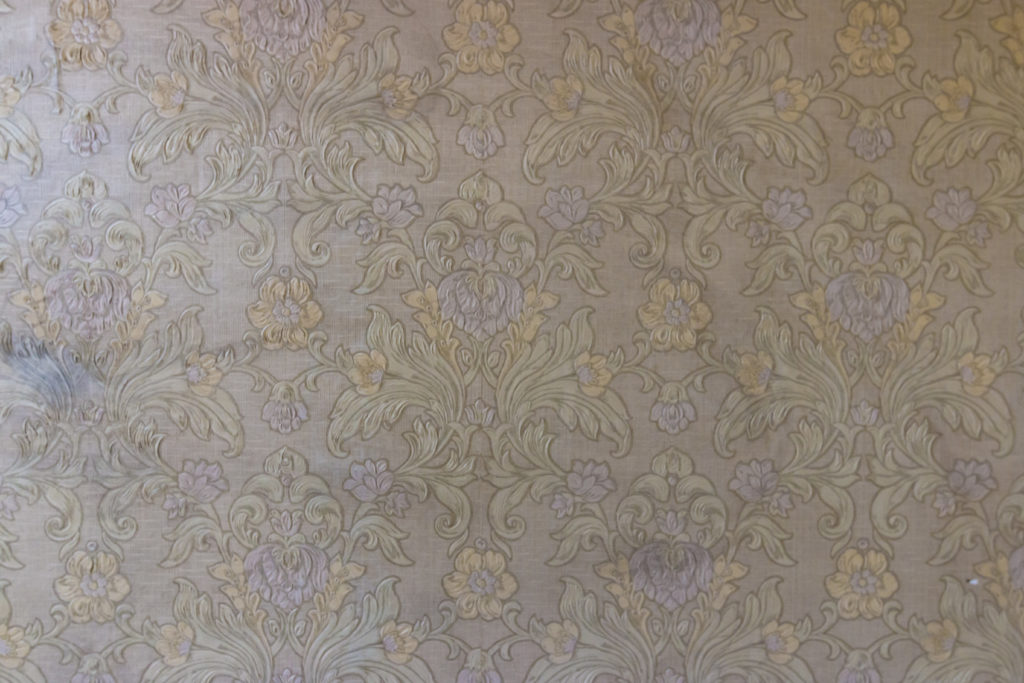
\includegraphics[height=1.05\paperheight]{tapete}
};	

% Image credit of background
\node[at=(current page.south east),xshift=-6.6cm,yshift=0.2cm]{%
	\footnotesize\color{white}};
\end{tikzpicture}

\begin{tikzpicture}[overlay,remember picture]
\fill[brown!60!white!90!blue] ([yshift=+5cm]current page.south west) rectangle (current page.south east);
\end{tikzpicture}%

\centering
\begin{tikzpicture}[]
   \node[inner sep=5pt] (conn) at (0,0.8){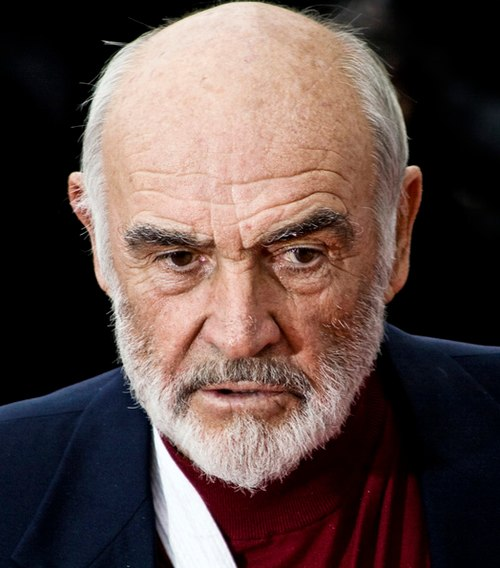
\includegraphics[width=2cm]{connery}};
   \fill[Ivory2](conn.south west) rectangle (conn.north east);	
   \draw[DarkGoldenrod2!80!black,line width=15pt] (conn.south west) rectangle (conn.north east);		
   \draw[brown!60!black,line width=10pt] (conn.south west) rectangle (conn.north east);
	%\draw[brown!60!black,line width=10pt] (current page.south east) rectangle (current page.north west);	
   \node at (0,0.8){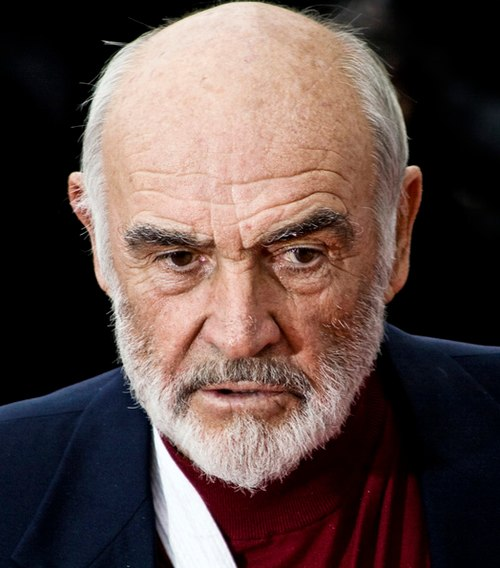
\includegraphics[width=2cm]{connery}};
\end{tikzpicture}%

\reflectbox{\usebox\bondducks}\qquad

\begin{tikzpicture}[scale=1.3,transform shape,baseline={(0,0)}]
  \mouse
  \begin{scope}[scale=0.6]
   \pic[rotate=40, local bounding box=microfono] at (1.2,1) {microph};
   \draw[black, line width=2pt] (microfono.-45) -- ++(-.2,+.2) ++(.2,-.2) -- ++(0,-1.5);
 \end{scope}
 \clip[rotate around={20:(-0.47,1.15)}] (-0.47,0.93) ellipse[x radius=0.13, y radius=0.24];
 \draw[black,line width=4pt,rotate around={20:(-0.47,1.15)}]  (-0.47,1.03) --++ (1,0)--++(-2,0);
\end{tikzpicture}
\usebox\bondducks

%
%\begin{tikzpicture}[baseline={(0,0)}]
% \bear
%   \foreach\x in {1,2,...,10}{
%  \ifodd\x \only<\x>{
% \fill[draw=brown!30!black,fill=brown,line width=0.4pt] (0.145, 1.38) arc [start angle=-20, end angle=-160, radius=0.16] -- cycle;}\else\only<\x>{} \fi}
%
% \begin{scope}[even odd rule]
%
%  \clip  (0, 1.55) circle (0.5)[reverseclip];
%  \clip  (0.425, 0.3) circle (0.28)[reverseclip];
%  \clip  (-0.425, 0.3) circle (0.28)[reverseclip];
%  \clip (-1,0.6) --++ (0.45,0)--++(-0.5,1) --cycle[reverseclip] ;
%  \clip ( 1,0.6) --++ (-0.45,0)--++(0.5,1) --cycle[reverseclip] ;
%  \clip(-1,0.5) rectangle (1,1.2);
%
%  \fill[europablau,rotate around={-50:(0.525,0.9)}](0.525,0.9) ellipse (0.35 and 0.15);
%  \fill[europablau,rotate around={50:(-0.525,0.9)}] (-0.525,0.9) ellipse (0.35 and 0.15);
%  \fill[europablau] (0,0.75) ellipse (0.55 and 0.65);
%  \fill[europablau] (0,0.7) ellipse (0.35 and 0.4);
%  \node at (0,0.8){\includegraphics[width=0.5cm,trim=2cm 0.7cm 2cm 0.7cm,clip]{flag_yellow_eps}};
%  \end{scope}
%\end{tikzpicture}
%%
%\begin{tikzpicture}[baseline={(0,0)},scale=1.15,transform shape,]
% \bear
%   \foreach\x in {1,2,...,10}{
%  \ifodd\x \only<\x>{
% \fill[draw=brown!30!black,fill=brown,line width=0.4pt] (0.145, 1.38) arc [start angle=-20, end angle=-160, radius=0.16] -- cycle;}\else\only<\x>{} \fi}
% \begin{scope}[even odd rule]
%
%  \clip  (0, 1.55) circle (0.5)[reverseclip];
%  \clip  (0.425, 0.3) circle (0.28)[reverseclip];
%  \clip  (-0.425, 0.3) circle (0.28)[reverseclip];
%  \clip (-1,0.6) --++ (0.45,0)--++(-0.5,1) --cycle[reverseclip] ;
%  \clip ( 1,0.6) --++ (-0.45,0)--++(0.5,1) --cycle[reverseclip] ;
%  \clip(-1,0.5) rectangle (1,1.2);
%
%  \fill[europablau,rotate around={-50:(0.525,0.9)}](0.525,0.9) ellipse (0.35 and 0.15);
%  \fill[europablau,rotate around={50:(-0.525,0.9)}] (-0.525,0.9) ellipse (0.35 and 0.15);
%  \fill[europablau] (0,0.75) ellipse (0.55 and 0.65);
%  \fill[europablau] (0,0.7) ellipse (0.35 and 0.4);
%  \node at (0,0.8){\includegraphics[width=0.5cm,trim=2cm 0.7cm 2cm 0.7cm,clip]{flag_yellow_eps}};
%  \end{scope}
%\end{tikzpicture}
%%
%\includegraphics{tartan}
%\begin{tikzpicture}[baseline={(0,0)}]
% \bear
%   \foreach\x in {1,2,...,10}{
%  \ifodd\x \only<\x>{
% \fill[draw=brown!30!black,fill=brown,line width=0.4pt] (0.145, 1.38) arc [start angle=-20, end angle=-160, radius=0.16] -- cycle;}\else\only<\x>{} \fi}
% \begin{scope}[even odd rule]
%
%  \clip  (0, 1.55) circle (0.5)[reverseclip];
%  \clip  (0.425, 0.3) circle (0.28)[reverseclip];
%  \clip  (-0.425, 0.3) circle (0.28)[reverseclip];
%  \clip (-1,0.6) --++ (0.45,0)--++(-0.5,1) --cycle[reverseclip] ;
%  \clip ( 1,0.6) --++ (-0.45,0)--++(0.5,1) --cycle[reverseclip] ;
%  \clip(-1,0.5) rectangle (1,1.2);
%
%  \fill[europablau,rotate around={-50:(0.525,0.9)}](0.525,0.9) ellipse (0.35 and 0.15);
%  \fill[europablau,rotate around={50:(-0.525,0.9)}] (-0.525,0.9) ellipse (0.35 and 0.15);
%  \fill[europablau] (0,0.75) ellipse (0.55 and 0.65);
%  \fill[europablau] (0,0.7) ellipse (0.35 and 0.4);
%  \node at (0,0.8){\includegraphics[width=0.5cm,trim=2cm 0.7cm 2cm 0.7cm,clip]{flag_yellow_eps}};
%  \end{scope}
%\end{tikzpicture}


%\begin{tikzpicture}[remember picture, overlay]
%\node at ({5.4+0.1*sin(\thepage)},{31.16-0.0472*(\thepage)}) {\includegraphics[width=\paperwidth]{snowflakes}};
%\end{tikzpicture}

\end{frame}
\end{document} 